\section{Base de Imagens} \label{pontosBaseImg}

Para a execução dos experimentos desta etapa do projeto serão utilizadas duas bases de imagens. Cada base, por sua vez, registra um objeto em diferentes ângulos num ambiente que possui níveis de iluminação extremos. Para cada ângulo do objeto, foram registradas imagens em diferentes tempos de exposição, para que assim possam ser utilizadas pelos métodos de geração de imagens HDR, e então gerar a nuvem de pontos como proposto na Seção \ref{pontosProposta}.

Para fins de comparação entre os processos propostos, para cada base de imagens, será discriminado um conjunto de imagens LDR mais bem expostas. Esse conjunto consiste na imagem de cada ângulo do objeto avaliada visualmente como sendo a mais bem exposta. E o mesmo será utilizado posteriormente para a obtenção de nuvem de pontos, que será comparada com as nuvens obtidas utilizando os métodos propostos.

\subsection{Base Controlada} \label{pontosBControl}
Esta base de imagens busca verificar o funcionamento dos métodos propostos numa situação próxima do ideal, i.e. onde há pouco ou nenhum movimento entre a captura de duas imagens de um mesmo ângulo do objeto. As imagens desta base são mostradas nas Figuras \ref{figBaseCFrente}, \ref{figBaseCDireita}, \ref{figBaseCEsquerda} e \ref{figBaseCCima}.

\begin{figure}[H]
  \centering 
  \subfloat[Tempo de exposição de $2ms$.]
  {
    \includegraphics[height=4cm]{Base1/Frente/1}
    \label{figBaseCFrenteA}
  }
  \quad %espaco separador
  \subfloat[Tempo de exposição de $4ms$.]
  {
    \includegraphics[height=4cm]{Base1/Frente/2}
    \label{figBaseCFrenteB}
  }
  \quad %espaco separador
  \subfloat[Tempo de exposição de $8ms$.]
  {
    \includegraphics[height=4cm]{Base1/Frente/3}
    \label{figBaseCFrenteC}
  }
  \quad %espaco separador
  \subfloat[Tempo de exposição de $17ms$.]
  {
    \includegraphics[height=4cm]{Base1/Frente/4}
    \label{figBaseCFrenteD}
  }
  \caption{Registro em diferentes tempos de exposição da frente do objeto.}
  \label{figBaseCFrente}
\end{figure}

\begin{figure}[H]
  \centering 
  \subfloat[Tempo de exposição de $2ms$.]
  {
    \includegraphics[height=4cm]{Base1/Direita/1}
    \label{figBaseCDireitaA}
  }
  \quad %espaco separador
  \subfloat[Tempo de exposição de $4ms$.]
  {
    \includegraphics[height=4cm]{Base1/Direita/2}
    \label{figBaseCDireitaB}
  }
  \quad %espaco separador
  \subfloat[Tempo de exposição de $8ms$.]
  {
    \includegraphics[height=4cm]{Base1/Direita/3}
    \label{figBaseCDireitaC}
  }
  \quad %espaco separador
  \subfloat[Tempo de exposição de $17ms$.]
  {
    \includegraphics[height=4cm]{Base1/Direita/4}
    \label{figBaseCDireitaD}
  }
  \caption{Registro em diferentes tempos de exposição da esquerda do objeto.}
  \label{figBaseCDireita}
\end{figure}

\begin{figure}[H]
  \centering 
  \subfloat[Tempo de exposição de $1,25ms$.]
  {
    \includegraphics[height=4cm]{Base1/Esquerda/1}
    \label{figBaseCEsquerdaA}
  }
  \quad %espaco separador
  \subfloat[Tempo de exposição de $3,13ms$.]
  {
    \includegraphics[height=4cm]{Base1/Esquerda/2}
    \label{figBaseCEsquerdaB}
  }
  \quad %espaco separador
  \subfloat[Tempo de exposição de $6,25ms$.]
  {
    \includegraphics[height=4cm]{Base1/Esquerda/3}
    \label{figBaseCEsquerdaC}
  }
  \quad %espaco separador
  \subfloat[Tempo de exposição de $12,5ms$.]
  {
    \includegraphics[height=4cm]{Base1/Esquerda/4}
    \label{figBaseCEsquerdaD}
  }
  \caption{Registro em diferentes tempos de exposição da direita do objeto.}
  \label{figBaseCEsquerda}
\end{figure}

\begin{figure}[H]
  \centering 
  \subfloat[Tempo de exposição de $1,25ms$.]
  {
    \includegraphics[height=4cm]{Base1/Cima/1}
    \label{figBaseCCimaA}
  }
  \quad %espaco separador
  \subfloat[Tempo de exposição de $3,13ms$.]
  {
    \includegraphics[height=4cm]{Base1/Cima/2}
    \label{figBaseCCimaB}
  }
  \quad %espaco separador
  \subfloat[Tempo de exposição de $6,25ms$.]
  {
    \includegraphics[height=4cm]{Base1/Cima/3}
    \label{figBaseCCimaC}
  }
  \quad %espaco separador
  \subfloat[Tempo de exposição de $12,5ms$.]
  {
    \includegraphics[height=4cm]{Base1/Cima/4}
    \label{figBaseCCimaD}
  }
  \caption{Registro em diferentes tempos de exposição da parte de cima do objeto.}
  \label{figBaseCCima}
\end{figure}

O conjunto de imagens selecionadas como sendo as mais bem expostas, para esta base de imagens, são as Figuras \ref{figBaseCFrenteC}, \ref{figBaseCDireitaC}, \ref{figBaseCEsquerdaC} e  \ref{figBaseCCimaB}.

\subsection{Base Capturada Manualmente} \label{pontosBLivre}

Esta base de imagens busca verificar o funcionamento dos métodos propostos numa situação convencional, i.e. onde o usuário captura as imagens manualmente sem ajuda de ferramentas profissionais como tripé ou software de captura. Isto implica na existência de movimento entre a captura de duas imagens de um mesmo ângulo do objeto. As imagens desta base são mostradas nas Figuras \ref{figBaseFrente}, \ref{figBaseDireita}, \ref{figBaseEsquerda} e \ref{figBaseCima}. 

\begin{figure}[H]
  \centering 
  \subfloat[Tempo de exposição de $1,25ms$.]
  {
    \includegraphics[height=4cm]{Base2/Frente/1}
    \label{figBaseFrenteA}
  }
  \quad %espaco separador
  \subfloat[Tempo de exposição de $8ms$.]
  {
    \includegraphics[height=4cm]{Base2/Frente/2}
    \label{figBaseFrenteB}
  }
  \quad %espaco separador
  \subfloat[Tempo de exposição de $20ms$.]
  {
    \includegraphics[height=4cm]{Base2/Frente/3}
    \label{figBaseFrenteC}
  }
  \quad %espaco separador
  \subfloat[Tempo de exposição de $100ms$.]
  {
    \includegraphics[height=4cm]{Base2/Frente/4}
    \label{figBaseFrenteD}
  }
  \caption{Registro em diferentes tempos de exposição da frente do objeto.}
  \label{figBaseFrente}
\end{figure}

\begin{figure}[H]
  \centering 
  \subfloat[Tempo de exposição de $0,8ms$.]
  {
    \includegraphics[height=4cm]{Base2/Direita/1}
    \label{figBaseDireitaA}
  }
  \quad %espaco separador
  \subfloat[Tempo de exposição de $5ms$.]
  {
    \includegraphics[height=4cm]{Base2/Direita/2}
    \label{figBaseDireitaB}
  }
  \quad %espaco separador
  \subfloat[Tempo de exposição de $33,3ms$.]
  {
    \includegraphics[height=4cm]{Base2/Direita/3}
    \label{figBaseDireitaC}
  }
  \quad %espaco separador
  \subfloat[Tempo de exposição de $125ms$.]
  {
    \includegraphics[height=4cm]{Base2/Direita/4}
    \label{figBaseDireitaD}
  }
  \caption{Registro em diferentes tempos de exposição da esquerda do objeto.}
  \label{figBaseDireita}
\end{figure}

\begin{figure}[H]
  \centering 
  \subfloat[Tempo de exposição de $0,8ms$.]
  {
    \includegraphics[height=4cm]{Base2/Esquerda/1}
    \label{figBaseEsquerdaA}
  }
  \quad %espaco separador
  \subfloat[Tempo de exposição de $6,25ms$.]
  {
    \includegraphics[height=4cm]{Base2/Esquerda/2}
    \label{figBaseEsquerdaB}
  }
  \quad %espaco separador
  \subfloat[Tempo de exposição de $25ms$.]
  {
    \includegraphics[height=4cm]{Base2/Esquerda/3}
    \label{figBaseEsquerdaC}
  }
  \quad %espaco separador
  \subfloat[Tempo de exposição de $125ms$.]
  {
    \includegraphics[height=4cm]{Base2/Esquerda/4}
    \label{figBaseEsquerdaD}
  }
  \caption{Registro em diferentes tempos de exposição da direita do objeto.}
  \label{figBaseEsquerda}
\end{figure}

\begin{figure}[H]
  \centering 
  \subfloat[Tempo de exposição de $1,56ms$.]
  {
    \includegraphics[height=4cm]{Base2/Cima/1}
    \label{figBaseCimaA}
  }
  \quad %espaco separador
  \subfloat[Tempo de exposição de $16,7ms$.]
  {
    \includegraphics[height=4cm]{Base2/Cima/2}
    \label{figBaseCimaB}
  }
  \quad %espaco separador
  \subfloat[Tempo de exposição de $40ms$.]
  {
    \includegraphics[height=4cm]{Base2/Cima/3}
    \label{figBaseCimaC}
  }
  \quad %espaco separador
  \subfloat[Tempo de exposição de $166,7ms$.]
  {
    \includegraphics[height=4cm]{Base2/Cima/4}
    \label{figBaseCimaD}
  }
  \caption{Registro em diferentes tempos de exposição da parte de cima do objeto.}
  \label{figBaseCima}
\end{figure}

O conjunto de imagens selecionadas como sendo as mais bem expostas, para esta base de imagens, são as Figuras \ref{figBaseFrenteC}, \ref{figBaseDireitaC}, \ref{figBaseEsquerdaC} e \ref{figBaseCimaC}.